\label{rotor_nacelle}

The variable rotor diameter, turbine power rating, and blade and chord distributions in this study also needed be accounted for in structural analysis.  To do so, we used a model developed at NREL called RotorSE  to calculate the rotor mass, rated and extreme thrust, rated torque, rated wind speed, and moments of inertia \citep{ning2013rotorse}. The complex nature of RotorSE allows the user to fully define a rotor and perform analysis, however this comes at a cost in computation time. Because we coupled turbine design and turbine layout optimization, the rotor analysis needed to be called many more times than in an isolated turbine design optimization. 
Thus, to speed up the rotor calculations in our optimization, we created a surrogate model on the results provided by RotorSE. We sampled rotor diameters evenly spaced from 46 meters to 160 meters, every six meters, and rated powers from 0.5 megawatts to ten megawatts, every 0.5 megawatts. The lower limits, 46 meter rotor diameter and 500 kilowatt rated power, are both lower than we expected any of the optimal values to be. The upper limits, 160 meter rotor diameter and 10 megawatt rated power are both near the upper limit of current wind turbine technology. For each combination of rotor diameter and rated power, we used RotorSE to minimize the blade mass using the blade chord and twist distributions as design variables. The optimization was constrained such that the turbine blades would not fail from stress or buckling and the power coefficient was greater than 0.42. Note that we did not vary the airfoils in the optimizations. 
We then used the converged optimizations, and used k-fold cross-validation with 10 groups to choose a fifth order bivariate spline which was then applied to each of the outputs of interest. This spline function was then used in place of RotorSE in our wind farm optimizations. By creating the surrogate, we achieved the accuracy of RotorSE without the large associated time requirement, as well as fast and simple analytic gradients. 
The k-fold cross-validation with 10 groups showed that the mean error is below 4\% for the moments of inertia, approximately 4.5\% for the extreme thrust, and below 3\% for the rest of the fits. 
Figure \ref{rotor_nacelle} shows the normalized surface fits for each of the variables of interest.


\begin{figure}[htbp]
  \centering
  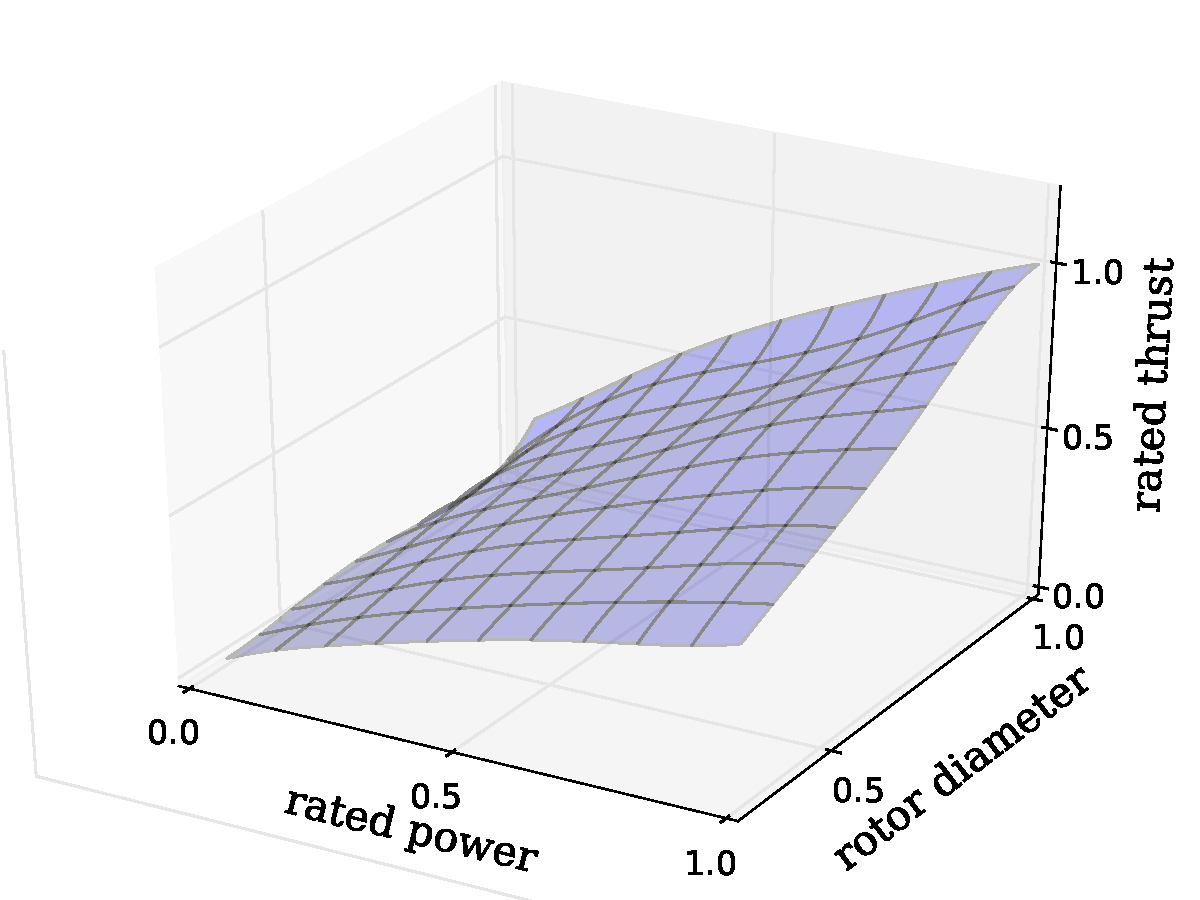
\includegraphics[trim={2cm 0 0 0},clip,width=0.33\textwidth]{Figures/rated_thrust.pdf}\label{rated_thrust}
  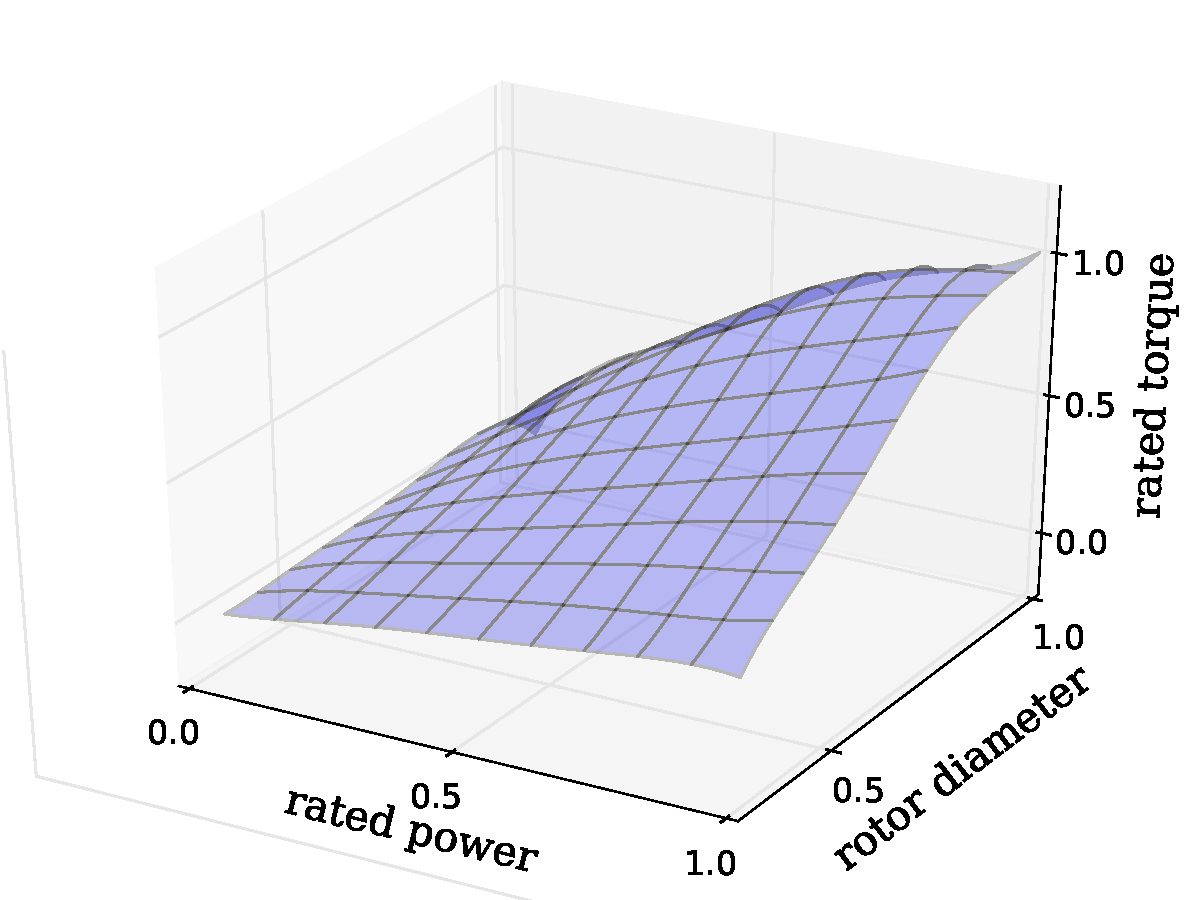
\includegraphics[trim={2cm 0 0 0},clip,width=0.33\textwidth]{Figures/rated_torque.pdf}\label{rated_torque}
 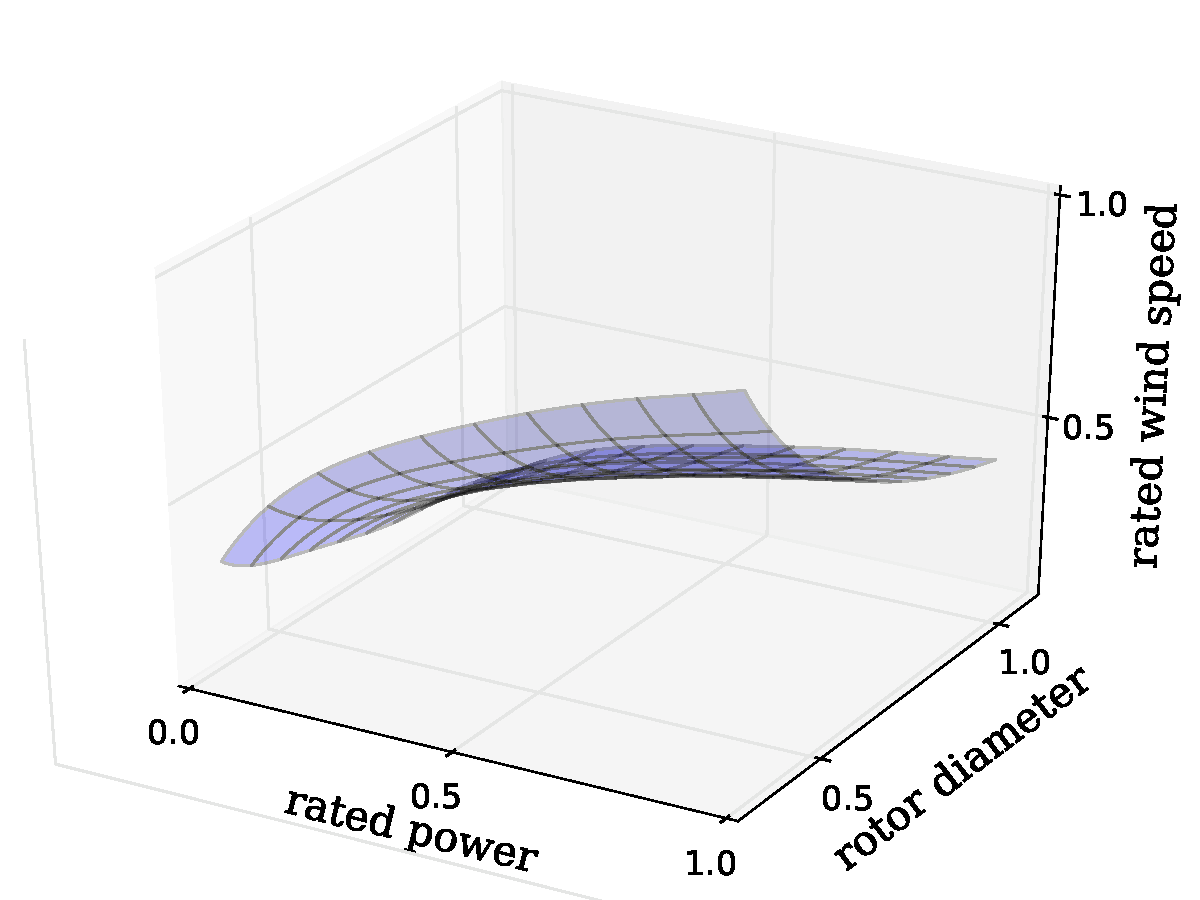
\includegraphics[trim={2cm 0 0 0},clip,width=0.33\textwidth]{Figures/rated_wind_speed.pdf}\label{rated_wind_speed}\\
  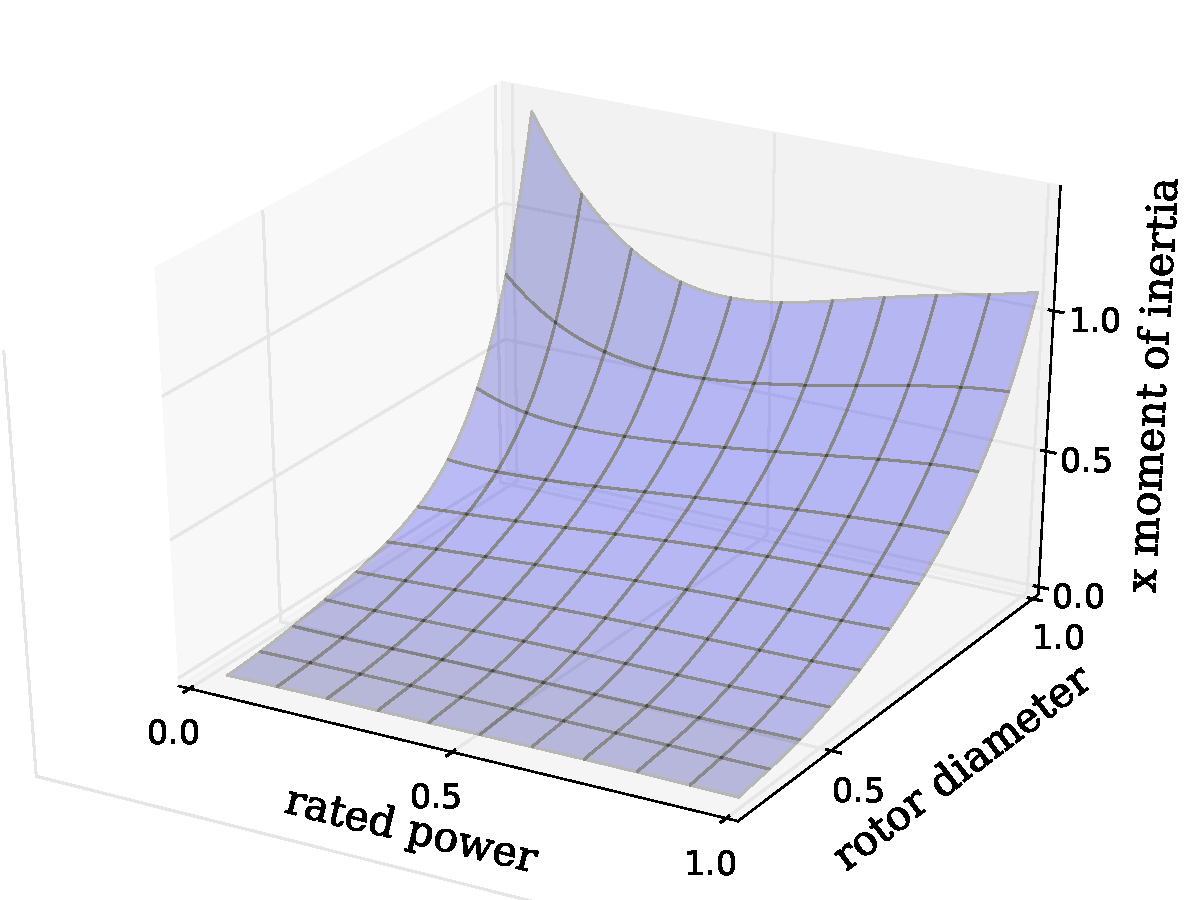
\includegraphics[trim={2cm 0 0 0},clip,width=0.33\textwidth]{Figures/x_mom_inertia.pdf}\label{xI}
  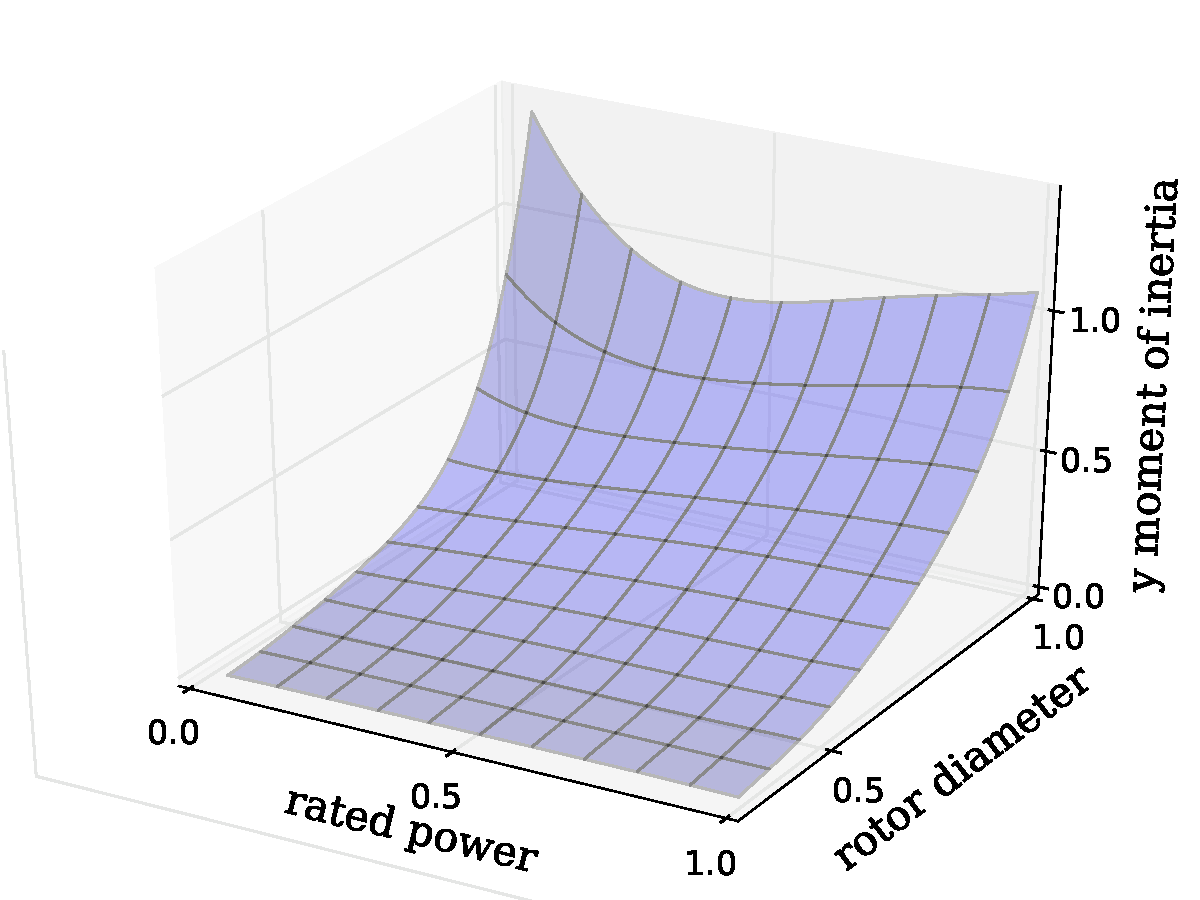
\includegraphics[trim={2cm 0 0 0},clip,width=0.33\textwidth]{Figures/y_mom_inertia.pdf}\label{yI}
  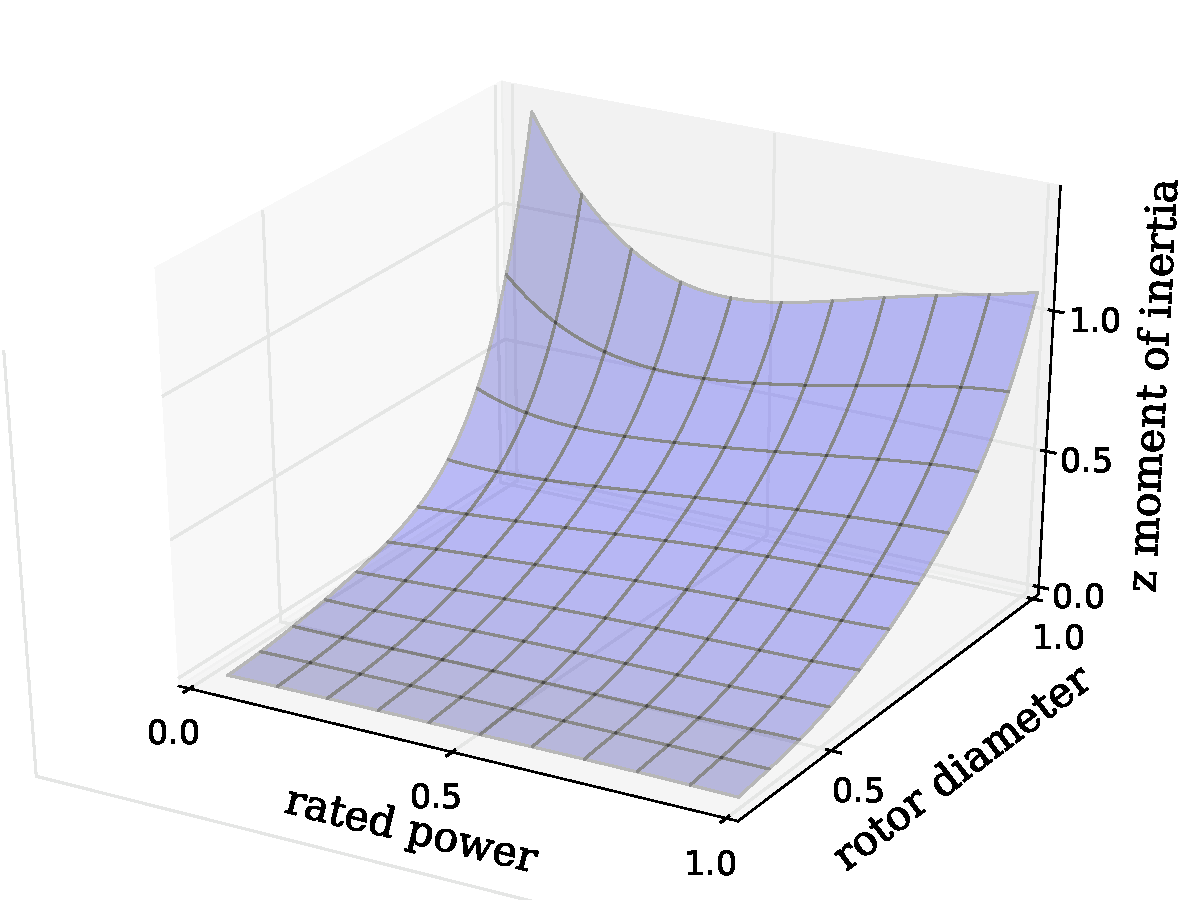
\includegraphics[trim={2cm 0 0 0},clip,width=0.33\textwidth]{Figures/z_mom_inertia.pdf}\label{zI} \\
 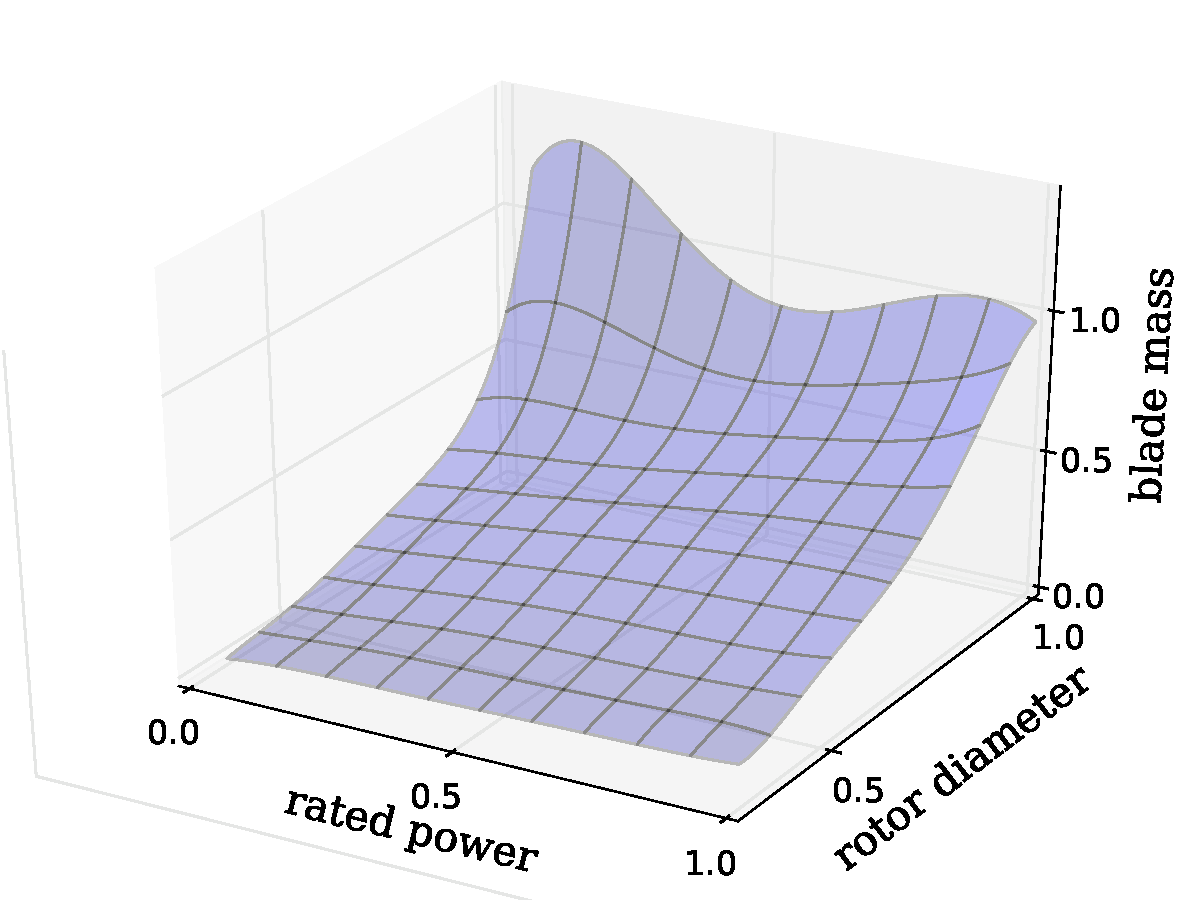
\includegraphics[trim={2cm 0 0 0},clip,width=0.33\textwidth]{Figures/blade_mass.pdf}\label{blade_mass}
 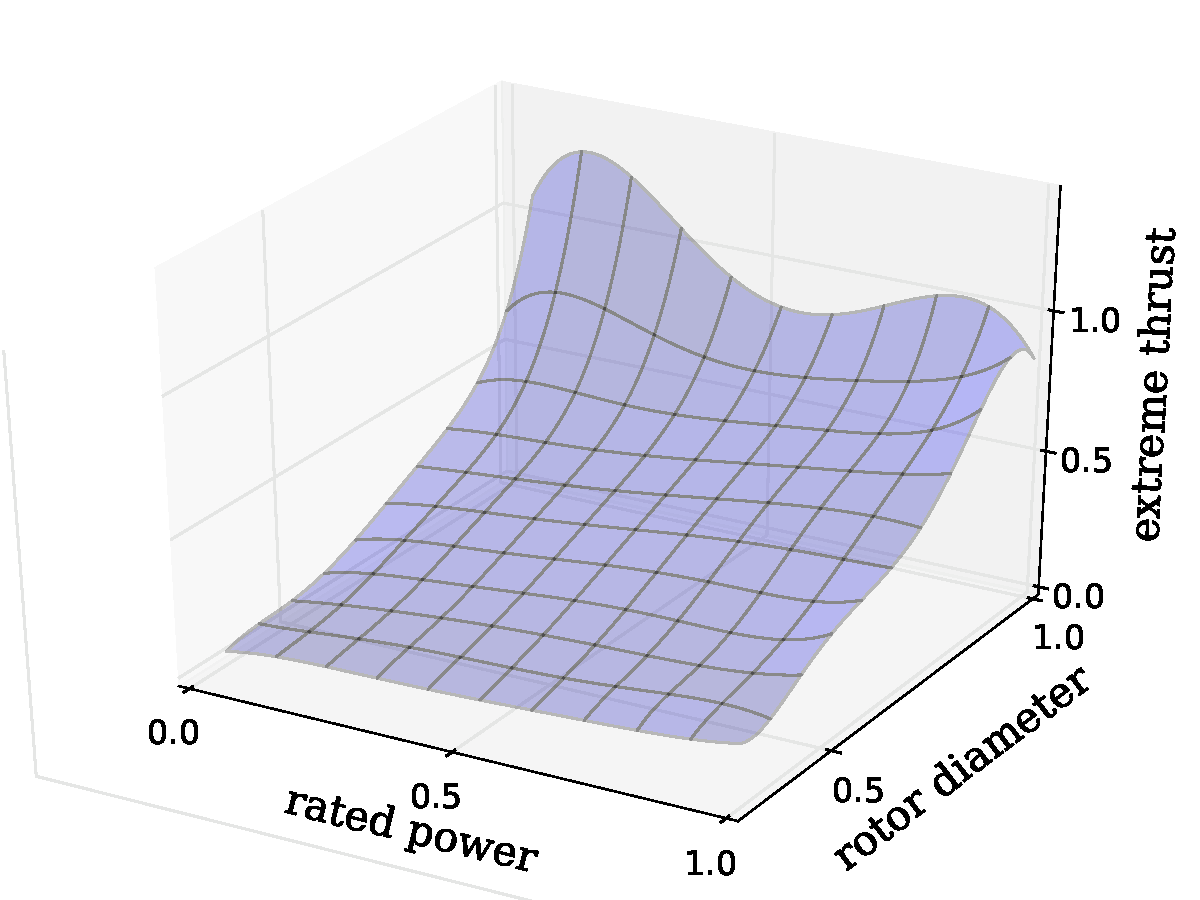
\includegraphics[trim={2cm 0 0 0},clip,width=0.33\textwidth]{Figures/extreme_thrust.pdf}\label{extreme_thrust}
  \caption{\label{rotor_nacelle} The spline fits to optimized RotorSE data. These fits were used to obtain the desired outputs of rotor mass, rated and extreme thrust, rated torque, rated wind speed, and moments of inertia as functions of the rotor diameter and rated power.}
\end{figure}